\section{Runtime View}\label{sec:runtime-view}

\subsection{OAuth 2.0 Authentication Flow}\label{subsec:oauth-2.0-authentication-flow}

The OAuth 2.0 authentication flow is a crucial component of the system's security infrastructure, ensuring that only authenticated and authorized users can access the application.
Figure~\ref{fig:oauth_sequence} illustrates the sequence of interactions during the OAuth 2.0 authentication process.

\begin{figure}[ht]
    \centering
    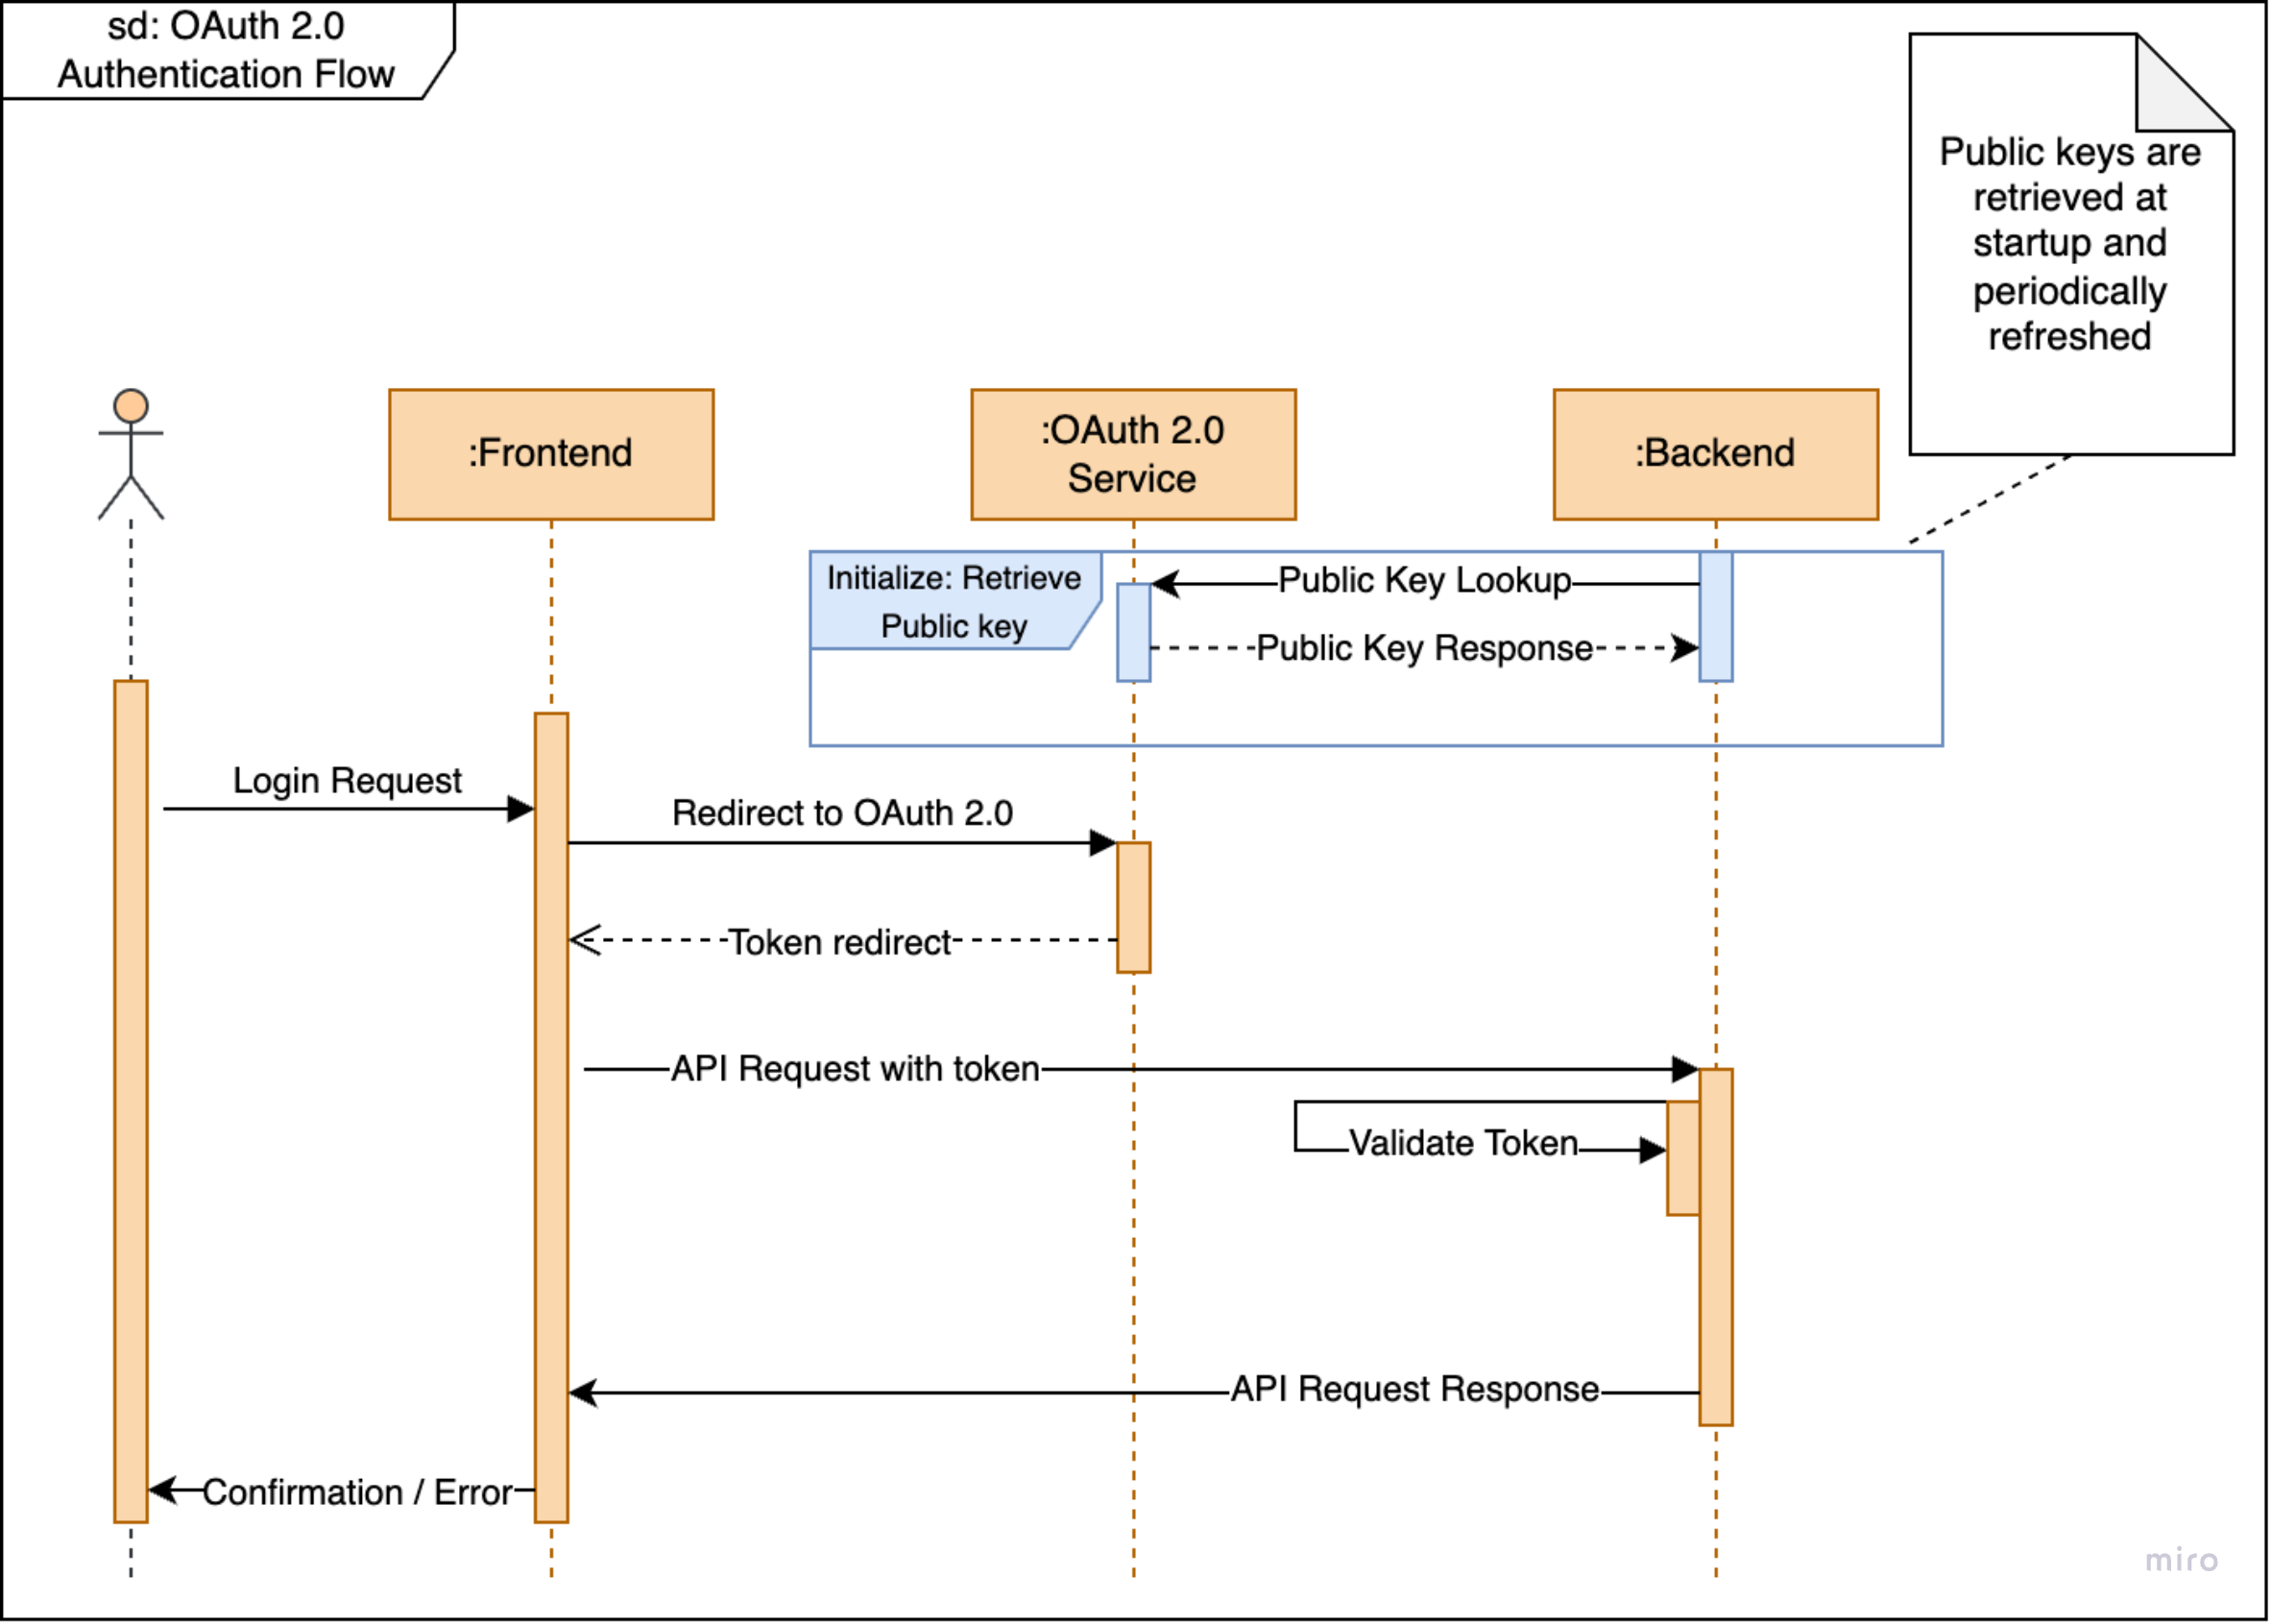
\includegraphics[scale=0.16]{images/high_level_architecture/authentication_flow}
    \caption{Sequence diagram of the OAuth 2.0 authentication flow}
    \label{fig:oauth_sequence}
\end{figure}

As the diagram depicts, the process begins with the user's request to log in, which leads to a series of interactions between the client application, the OAuth 2.0 service, and the backend server. This interaction sequence ensures a secure exchange of credentials and tokens, maintaining the integrity and confidentiality of the authentication process.

\subsection{Runtime Scenario 2}\label{subsec:runtime-scenario-2}
TODO